\documentclass[12pt]{article}

\usepackage{graphicx}
\usepackage{float}
\usepackage{amsmath}
\usepackage{amsfonts} 
\usepackage{hyperref}
\usepackage{color}
\usepackage{pagecolor}
\usepackage[most]{tcolorbox}
\usepackage{tikz}
\usepackage{pgf-pie}
\usepackage{xcolor}


\textheight = 20 cm

\definecolor{blueColor}{HTML}{0069f5}

\begin{document}

\newpage

\pagecolor{blueColor}

\begin{titlepage}
    \centering

     
\includegraphics[width=0.88\textwidth, keepaspectratio]{latex-cover.png}
    
\end{titlepage}

\newpage

\pagecolor{white}

\renewenvironment{abstract}
 {\small
  \begin{center}
  \bfseries \abstractname\vspace{-.5em}\vspace{0pt}
  \end{center}
  \list{}{
    \setlength{\leftmargin}{.5cm}
    \setlength{\rightmargin}{\leftmargin}
  }
  \item\relax}
 {\endlist}
 

\title{\textbf{Adabuy:\\A P2P e-commerce protocol based on trust rating and mediators }}

\author{Juan C. Rey\footnote{Repository: \url{https://github.com/adabuy/core} - Plutus Pioneer First Cohort. This is a work in progress since 2023 for the Cardano open source community.  }\\} 

\maketitle

\renewcommand*\abstractname{\textbf{}\hfill}

\abstract{
\textbf{Abstract.}
Adabuy is an electronic commerce protocol that uses smart contracts to decentralize functional requirements necessary for the processes of selling and buying a physical product.
Any member of the community can post a product for sale and any member of the community can express an intention to purchase that product. During a negotiation session the buyer and seller generate the context by engaging in bilateral communication through live chat via websocket.
If a dispute arises during the session it is possible to appeal so that a mediator can decide on the specific case in accordance with the fulfillment of the obligations of the buyer and the seller. The fundamental idea behind Adabuy is to avoid using expensive tracker hardware and infrastructure as a source of truth. Instead, use mediators to resolve unsuccessful product negotiations. To encourage users to buy from Adabuy instead of the traditional marketplace, a liquidity pool helps create discounts on best-selling products. The liquidity pool is a way to return the money from the fees to the users and sell the products cheaper with a discount. A very effective feature to compete with the traditional market that collects a large percentage of commissions on the sale of products and are not returned.

}

 
\section{Introduction}

\begin{figure}[ht]
  \centering
  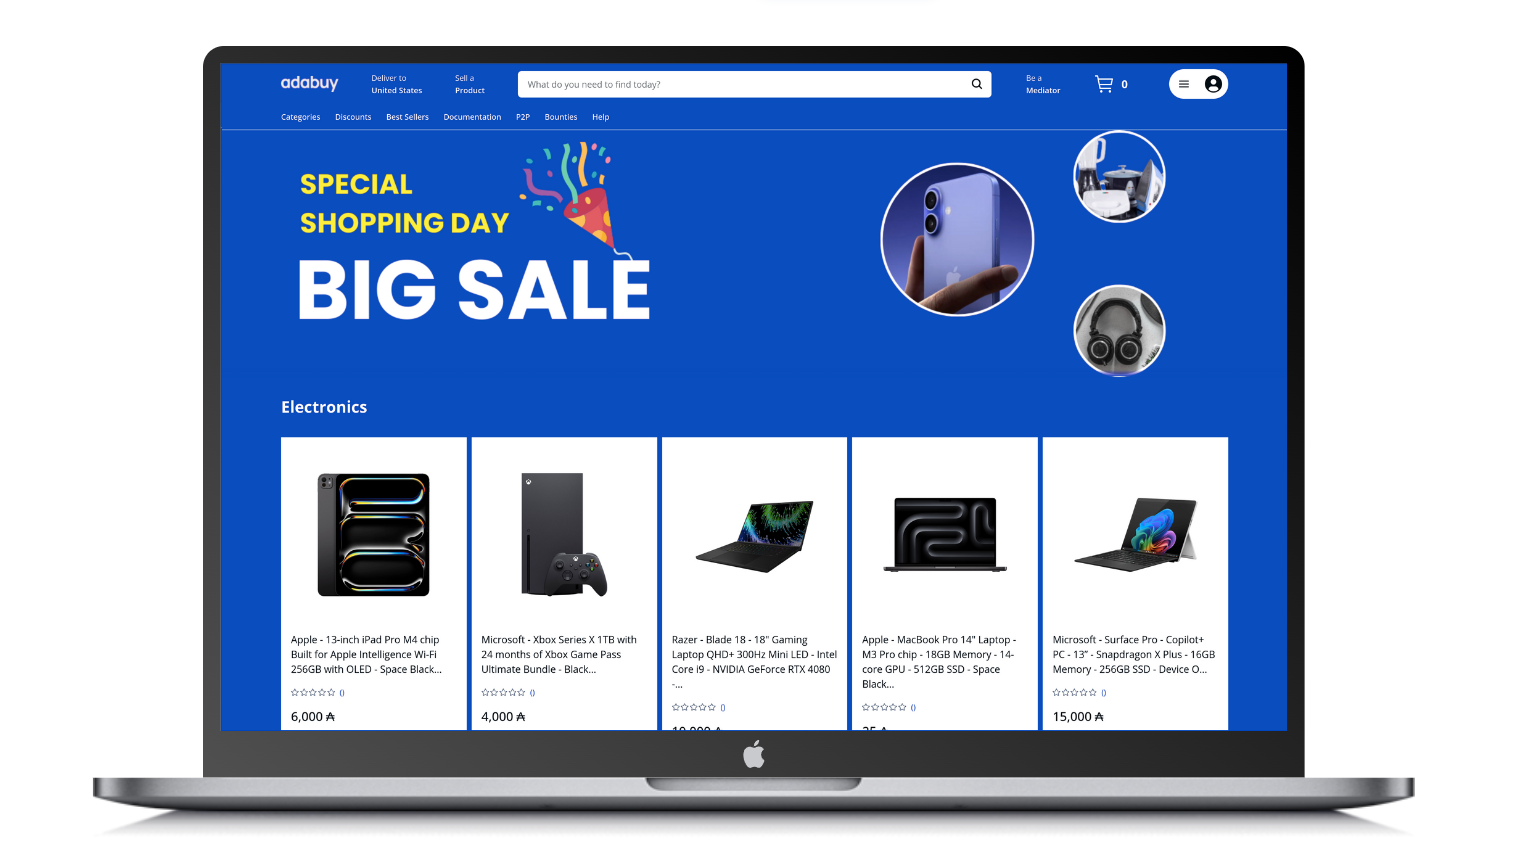
\includegraphics[width=0.88\textwidth, keepaspectratio]{adabuy.png}
  \caption{Cardano native marketplace}
  \label{fig:web}
\end{figure}

A completely decentralized e-commerce protocol can be described as trading in physical products or services where parties use digital devices and blockchain to fulfill their obligations.
The seller's obligation is to deliver the product or service and the buyer's obligation is to pay the price corresponding to the product or service. 
The entire process can be digital if the product or service is digital.
Regarding physical products it is necessary to use the service of shipping companies to physical destinations.
To apply blockchain to the physical process of delivering a product it is necessary to establish a digital channel that provides infallible information about the delivery of the product and therefore the fulfillment of the seller's obligation. 

The main problem with adding blockchain to an e-commerce is the expensive use of hardware trackers that determine whether a product was delivered to the buyer or not in cases of dispute. These devices should theoretically provide all the information via chain, which represents technical challenges such as scalability, constant internet connection, computer manipulation, interference, etc. There is another way to ensure the truth about whether a product was successfully delivered to the buyer without using hardware. With a P2P system with appeals like the one Binance uses for transactions between people using physical bank accounts. This system can be applied to Adabuy for the negotiation of products and ensures that there is a fair resolution of conflict cases.

Peer-to-Peer cryptocurrency exchange services such as localbitcoins or binance P2P have proven to be systems that work for secure trades. These systems are based on trust rating and involve real-world action on the part of the buyer such as making a transaction to the bank account provided by the seller. In Binance P2P, disputes between buyers and sellers can be addressed through an appeal process. Common reasons for initiating an appeal involves problems with payment confirmation, disagreements over payment quality, or disputes regarding trade terms. To protect the cryptocurrency involved in the trade an escrow system locks the funds.

Both the buyer and seller are afforded the opportunity to present evidence or explanations supporting their case during the appeal. A mediation team at Binance reviews the appeal carefully considering the evidence and arguments put forth by both parties. Subsequently, Binance reaches a decision which may involve upholding the original trade agreement, releasing funds from escrow to the appropriate party, or taking other actions based on the specific circumstances of the dispute. In ADABUY this role is performed by mediators who decide on appeals.

Binance reached approximately 170 million registered users by the end of 2023. A large percentage of users carry out P2P negotiations using bank accounts and physical world payment methods. Binance has demonstrated that the Peer-to-Peer exchange system with appeal mechanism is effective and scalable.

If a dispute arises during the session it is possible to appeal so that a mediator can decide on the specific case in accordance with the fulfillment of the obligations of the buyer and the seller. The fundamental idea behind Adabuy is to avoid using expensive tracker hardware and infrastructure as a source of truth in those cases which in principle are the minority. Instead, use mediators to resolve unsuccessful product negotiations.

Adabuy aims to be one of the first Dapps on Cardano to materialize one of the most important blockchain use cases and compete with the traditional market by offering innovation and benefits to users by taking advantage of Cardano's Turing-complete contracts. The possibilities for innovation exceed traditional marketplaces. One of its strengths is its liquidity pool so that fees become discounts on the top products most requested by the community. 
A very effective feature to compete with the traditional market that collects a large percentage of commissions on the sale of products and are not returned. Adabuy is designed to scale horizontally using microservices and its code is completely open-source.
Product prices are shown in USD but at the time of payment the conversion to ADA is made, this allows prices to be compared to the traditional market. Cardano's transactional layer allows to Adabuy trading in ADA and in the future also with \underline{stablecoins} that run on this network which is exciting.

\section{ Protocol and Patterns }

Two design patterns have been identified that are fundamental to the successful and effective implementation of Adabuy.

\subsection { The Seller Pattern. } 

In this design the seller takes the first step by deploying the plutus V3 script to the Cardano blockchain so that eventually in the future buyers will interact with those scripts. This pattern has 4 stages \emph{Waiting}, \emph{Locking}, \emph{Shipping}, \emph{Delivered}.

\subsubsection { Waiting }

When a seller offers a product to the public by activating a sell order a small Plutus V3 script with state machine logic is activated in the blockchain.
The seller must lock an amount greater than 0 ADA as collateral. 
If the seller acts in bad faith during the negotiation session the seller will lose the collateral.
If the seller is a good agent during the negotiation session the collateral will return to him.
Collateral guarantees that the seller behaves honestly.
This mechanism of coercion allows to generate trust in potential buyers. 
It also allows the seller to increase their trust rating. Example. Alice publishes a book with 20 units of stock.
She activates only 10 sell orders each with a collateral of 20 ADA.
In the first few hours 7 books were sold and now there are only 3 orders left.
Alice decides to activate the 10 remaining orders due to demand.
Bob sells the same product with the same stock but offers collateral of 5 ADA. The community prefers to buy the books from Alice since she is more committed to fulfilling her obligation by offering 20 ADA collateral.

\begin{figure}[ht]
  \centering
  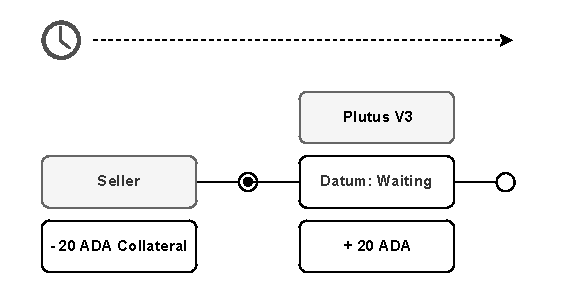
\includegraphics[width=0.88\textwidth, keepaspectratio]{1.pdf}
  \caption{Script deployment}
  \label{fig:mi_imagen}
\end{figure}
Other factors increase the seller's trust rating such as the total number of successful sales, seniority, or profile information.
In the background for each activated order individual scripts are deployed on the blockchain waiting to be occupied by buyers.
\\
\\
\\

\subsubsection { Locking } 

In figure 3 you can see the collateral of 20 ADA given by the seller and the price of the product 100 ADA given by the buyer.
When the buyer presses the buy button a order is occupied and the state of the script transitions from \emph{Waiting} to \emph{Locking}.
Blocking funds allows participants to advance their obligations.
The seller's obligation is to deliver the correct product with the correct specifications. The buyer's obligation is to receive the product.
It is important to clarify that the buyer's obligation to pay the price is guaranteed when he occupies a order since the amount in ADA of the product price is a necessary condition to occupy a order.

From this point the seller can start with questions such as: What is the delivery point? Description of delivery point? Any questions necessary to guarantee the effective delivery of the product.

All information provided by both actors in the user interface is contained within a websocket instance and can only be observed by the mediators in case of a dispute.
The websocket server does not store any type of information about the negotiation session once legal certainty is declared about the business between the parties.
Legal certainty is declared by the mediators and refers to the absence of reasonable doubt regarding compliance with the obligations that correspond to the buyer and the seller.

\begin{figure}[ht]
  \centering
  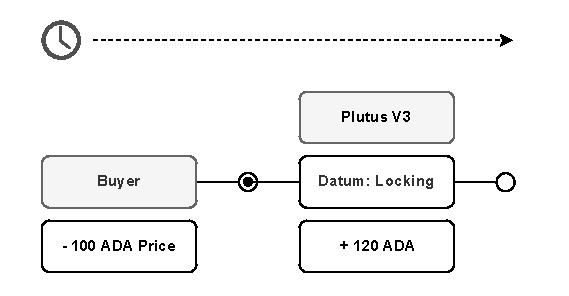
\includegraphics[width=0.88\textwidth, keepaspectratio]{2.pdf}
  \caption{Session locked}
  \label{fig:locking}
\end{figure}

\subsubsection { Shipping }

When the seller is notified that a buyer has purchased a sell order he must complete the process of shipping the product using a shipping company. When this becomes effective the seller will then need to press the @shipping button in the user interface.

\begin{figure}[ht]
  \centering
  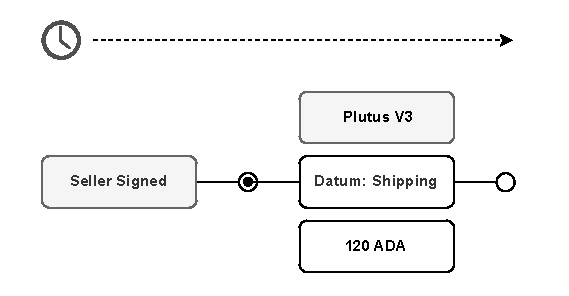
\includegraphics[width=0.88\textwidth, keepaspectratio]{3.pdf}
  \caption{The package has been sent.}  
  \label{fig:delivered}
\end{figure}
The script transitions from \emph{Locking} to the \emph{Shipping} state which indicates that the seller has fulfilled its shipping obligation. At this stage both the buyer and the system are notified that the product is en route and the buyer can start tracking the package via the provided tracking information.

\subsubsection { Received }

\begin{figure}[ht]
  \centering
  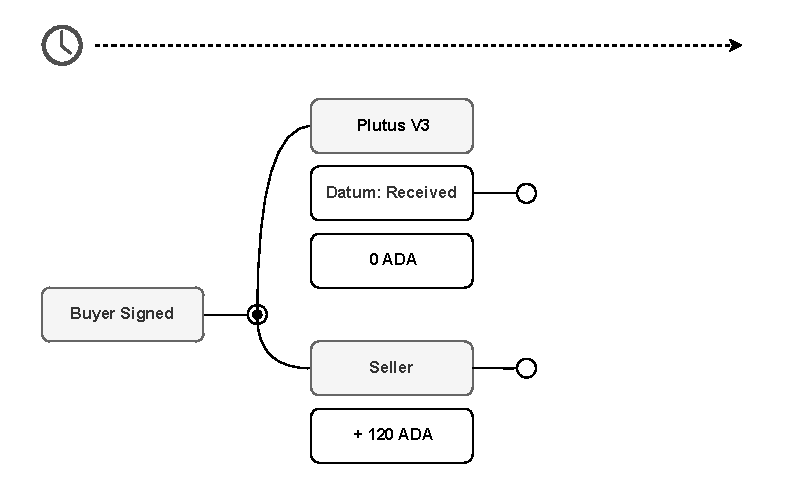
\includegraphics[width=0.88\textwidth, keepaspectratio]{4.pdf}
  \caption{The package has been received.}
  \label{fig:delivered}
\end{figure}

Finally the buyer confirms whether he received the product by invoking the @received endpoint. By doing so, the script transitions to the last state \emph{Received} which releases the funds to the seller's wallet. The seller receives 20 ADA of collateral and 100 ADA equivalent to the price of the product he sold to the buyer.

\subsubsection { Disadvantages }

The main disadvantage of this pattern is that scripts can last a long time without being taken up by buyers.
This means more resource consumption on the backend watching the script state. The seller may need to change prices frequently. The conversion from USD to ADA occurs when the seller deploys the script and not at the time of purchase. All these problems are solved with the Buyer Pattern explained below.
 
\subsection { The Buyer Pattern. } 

\subsubsection { Pending }

When the buyer sees a product and makes the purchase action the CBOR transaction is built in the backend containing everything needed for the trade. The backend also makes the respective USD to ADA appraisal corresponding to the price of the product. The backend checks to see if the transaction is validated by the nodes using the associated ThreadToken. When the transaction is confirmed the backend notifies the seller to accept the trade. If he decides not to accept it, then the buyer can claim his money back from the script. On the other hand, if the seller decides to accept the trade then they must provide the collateral and deliver the product. At this stage the buyer's funds are secured by a time logic and only the seller with the specific PubKeyHash can interact with the script.

\subsubsection { Locking }

At this stage the seller is notified via the user interface, email, and telegram of the purchase of a published product. The seller accepts on time and the backend builds a CBOR transaction that allows interaction with the script previously deployed by the buyer which has a set time for the seller to accept. The transaction contains a small collateral that affirms the seller's commitment to the trade. When the transaction is confirmed the contract goes into the \emph{Locking} state. After this moment the funds are blocked and the seller must send the product before the deadline is met.

\subsubsection { Shipping }

At this stage the seller ships the product and presses the "Shipped" button which builds a simple CBOR transaction that changes the script status to \emph{Shipping}. When the transaction is confirmed the buyer is notified of the shipping status and the corresponding information.

\subsubsection { Received }

At this stage the package has an approximate arrival date. When this date is reached, the buyer must notify the  the arrival of the package within a certain time. If he does not notify or APPEAL, then the trade of the product/s will be deemed completed and the funds will be released to the seller.

\subsection { State machine }
A state machine also known as a finite state machine (FSM), is a mathematical model used to describe the behavior of a system or process that can exist in a limited number of distinct states. The system transitions from one state to another in response to specific events or input conditions and these transitions are defined by a set of rules or conditions known as transitions.

A deterministic finite state machine (DFSM) is a specific type of state machine that exhibits deterministic behavior, meaning that for any given state and input there is a unique and unambiguous next state. In a deterministic state machine, the transition from one state to another is uniquely determined by the current state and the input with no ambiguity or randomness involved.

\begin{figure}[ht]
  \centering
  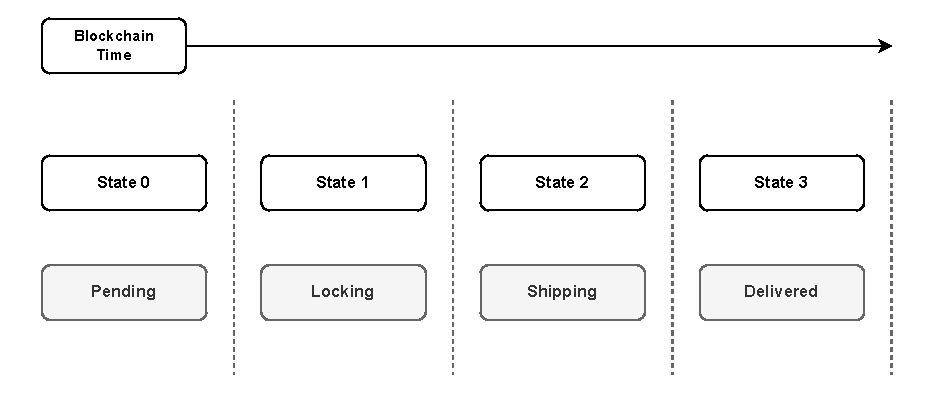
\includegraphics[width=0.95\textwidth]{machine.pdf}
  \caption{Session states}
  \label{fig:States}
\end{figure}
Figure 7 shows the deterministic state machine concepts applied to the steps of a negotiation session. 
The EUTXO model of the Cardano blockchain implies that smart contracts need an initial transaction for their logic to be activated and establish their initial state.

\subsection { Mediators }  

Connecting the blockchain to the real world is an expensive challenge at least for trading physical products.
Shipping companies would have to connect their vehicles to supervised oracles and the products must have an infallible tracker to check if were delivered.
A lot of infrastructure deployed around the world is necessary to achieve a fully decentralized ecommerce protocol.
Clearly this represents a very difficult challenge to achieve in contrast to another option which is to use the human as a source of truth.
With the right conditions the human can make logical reasoning about facts or propositions to declare a truth.
For example, the peer review system in the academic world allows a research paper to be reviewed by randomly assigned experts.
A blind reviewer does not know who is the author of the paper he is reviewing and the author also does not know who the reviewers are.
The system maintains confidentiality to prevent biases, ensuring a rigorous and impartial assessment. Serving as a crucial quality control mechanism, it identifies errors, provides constructive feedback to authors and contributes to the overall accuracy and reliability of published work. 
A system of blind peers trained in conflict resolution can decide on a dispute in a negotiation session in the event that the buyer or seller fails to comply with their obligations or another problem arises that does not allow the natural conclusion of the session.
A blind peer system can decide on a disputed trading session.

Some characteristics of the profile of a mediator are:

1. Mediators must stay neutral and impartial to ensure a fair and unbiased assessment of disputes fostering trust in the mediation process for all parties involved.

2. Effective communication is vital for mediators, involving active listening, skillful facilitation of discussions and clear conveyance of information to aid parties in mutual understanding and resolution.

3. A mediator needs strong problem-solving skills to navigate complex disputes and find mutually acceptable solutions. 

4. Mediators require patience as mediation processes take time, allowing parties to express themselves, explore solutions and reach agreements at their own pace.

5. Mediators must uphold ethical standards ensuring the confidentiality of the mediation process to establish and maintain the crucial element of trust for successful resolution.

6. Mediators require a comprehensive skill set encompassing technical, legal, and cultural knowledge to effectively carry out their duties.

\subsection { Appeal } 

\emph{Peer-to-Peer} cryptocurrency exchange services such as localbitcoins or binance P2P have proven to be systems that work for secure trades. These systems are based on trust rating and involve real-world action on the part of the buyer such as making a transaction to the bank account provided by the seller. In Binance P2P, disputes between buyers and sellers can be addressed through an appeal process. Common reasons for initiating an appeal involves problems with payment confirmation, disagreements over payment quality, or disputes regarding trade terms. To protect the cryptocurrency involved in the trade an escrow system locks the funds. Both the buyer and seller are afforded the opportunity to present evidence or explanations supporting their case during the appeal. A mediation team at Binance reviews the appeal carefully considering the evidence and arguments put forth by both parties. Subsequently, Binance reaches a decision which may involve upholding the original trade agreement, releasing funds from escrow to the appropriate party, or taking other actions based on the specific circumstances of the dispute.

In the case of Adabuy the seller is the party that has control over the terms of the negotiation. The UI view of a published product contains the product description, seller name, seniority, trust rating, number of successful sales, number of total sales, and the terms that any buyer must meet to be able to negotiate with the seller. These terms must be clear, enumerated and determined. Any buyer who accepts the seller's terms must comply with them. If the buyer does not comply with his obligation to receive the product the seller can initiate the appeal. Both parties can resort to appeal in case of dispute, a group of blind mediators can take action on a case-by-case basis.

The negotiation of a product generates a context and this can be validated using digital, visual or documentary evidence. The seller must provide visual evidence of the package and its contents before sending it. Evidence such as videos and photos of its packaging, reference labels, brands, receipt by the shipping company. In the case of dropshipping sellers, videos of their shipping process on the platform and supplier information. Documentary evidence of shipping receipts and shipping certificates are important. The seller must provide the valid guide number to monitor the package.

\subsection { Scalability } 

According to the principle of least cardinality in data modeling which states that one-to-many relationships such as between the author and the $N$ of published posts, the identifier that relates them should be stored on the ``many" side. In other words, when data modeling is designed posts should store the author identifier, authors should not store identifiers about their posts. As long as the author has a small number of published posts there are no problems with storing and consulting the information. The problem arises when the author has a large number of published posts, the storage of post identifiers in one of the author variables represents a scaling problem and the query time can be affected.
The application of this principle in the protocol architecture allows high horizontal scalability and the design of the plutus scripts. Scripts being individual do not depend on a main contract and execute their logic independently. This allows for high transaction batches per second. This architecture allows for high horizontal scalability and availability. Each service-gateway-1, service-gateway-2,3,4... contains several routes that build transactions in CBOR and are sent to the browser to be signed and sent by the user. The state service finds out about the new order and starts checking its status on the blockchain using the providers. In this way, the status is communicated to the other services and finally to the users.
\begin{figure}[ht]
  \centering
  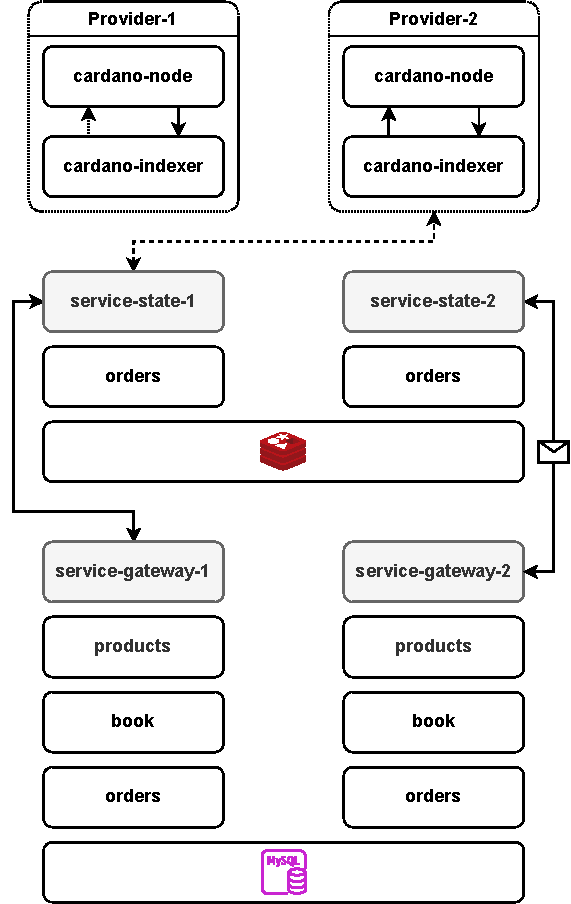
\includegraphics[width=0.5\textwidth]{horizontal.drawio.pdf}
  \caption{Horizontal Microservices}
  \label{fig:microservices}
\end{figure}
\\
Sharding databases allow for unlimited horizontal nodes to be added and Kubernetes allows for orchestrated management of unlimited pods. This type of architecture is known as event-driven microservices. Cardano acts as a decoupled transactional layer from this, allowing smart contracts to be interacted with from any source other than Adabuy if the contract allows it.

\subsection { Governance/Utility Token} 

The community using governance can change the policies and parameters of the protocol. For example: who meets the characteristics to be a mediator or not between the candidates. The token can also be assigned as utility such as visibility for the products. In this case, the product timeline/feed/views should be grouped to be fair to sellers who do not use the token.


\subsection { Liquidity Pool }

Each transaction on Adabuy generates a commission that goes to a liquidity pool. This pool has the function of treasury to pay for the infrastructure and the mediators.
The transaction commission must comply with these principles: It must always benefit the buyer. It must not be repulsive. It must be lower than that of the competition. Therefore, if 10,000 transactions occur with commissions of 0.5 ADA, then 2,500 ADA can go to discounts returning to users and 2,500 ADA to pay for technological infrastructure and mediators. 

To create discounts on products using money from the liquidity pool the best-selling published products will eventually have a discount tag. The buyer will pay the discounted price and when the delivery is completed the amount in ADA of the product price with the discount will be sent to the seller and finally a transaction from the liquidity pool will cover the shortfall of the original price of the product.

\subsection{ UI/UIX }

\subsubsection { Product } 

Any member of the community can publish a product only if they meet the following conditions:

1. Cannot be published any object, substance, biological, physical matter in any of its states and forms, declared illegal or prohibited by any type of international, state, federal, local or other regulations on the subject.

2. Comply with international, state, federal, local or other regulations on money laundering and drug trafficking.

3. Only physical products can be published, publication of services is not allowed.

4. Know and understand the licenses associated with the product.

5. Write in a specific and enumerated way the terms and conditions that the buyer must comply with.

6. Product must meet safety standards, must not pose a threat to the health or safety of the consumer.

7. Buyer have the right to be informed about the terms and conditions of a transaction, warranties, and return policies.

8. Comply with all international, state, federal, local and any regulations that regulate intellectual property rights.

9. Description of the product in a determined, fair, exact and precise manner.

10. Send the product with a recognized shipping company that allows tracking service.

In the user interface the product view must have the name of the product, the description of the product, the terms of the seller, the number of total sales of the seller, the number of successful sales of the seller, information about the seller, the stock number of the product, the number of activated orders, amount of ADA as collateral and trust rating. In the backend of the protocol there must be an automated service in charge of verifying the products before they are visible to the community.
\begin{figure}[ht]
  \centering
  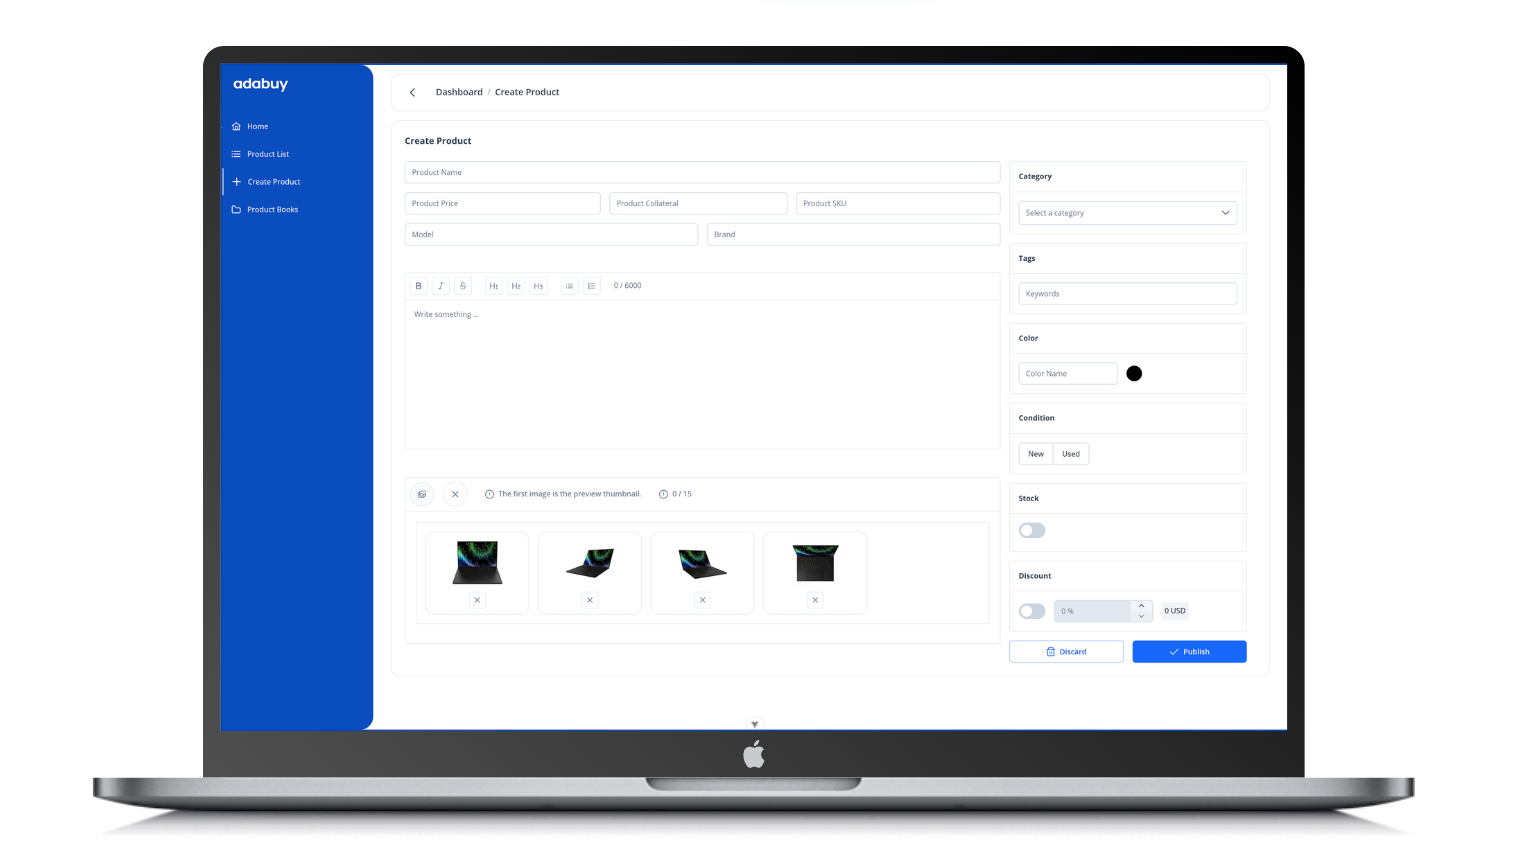
\includegraphics[width=0.88\textwidth, keepaspectratio]{create-product.png}
  \caption{Create}
  \label{fig:web}
\end{figure}

\begin{figure}[ht]
  \centering
  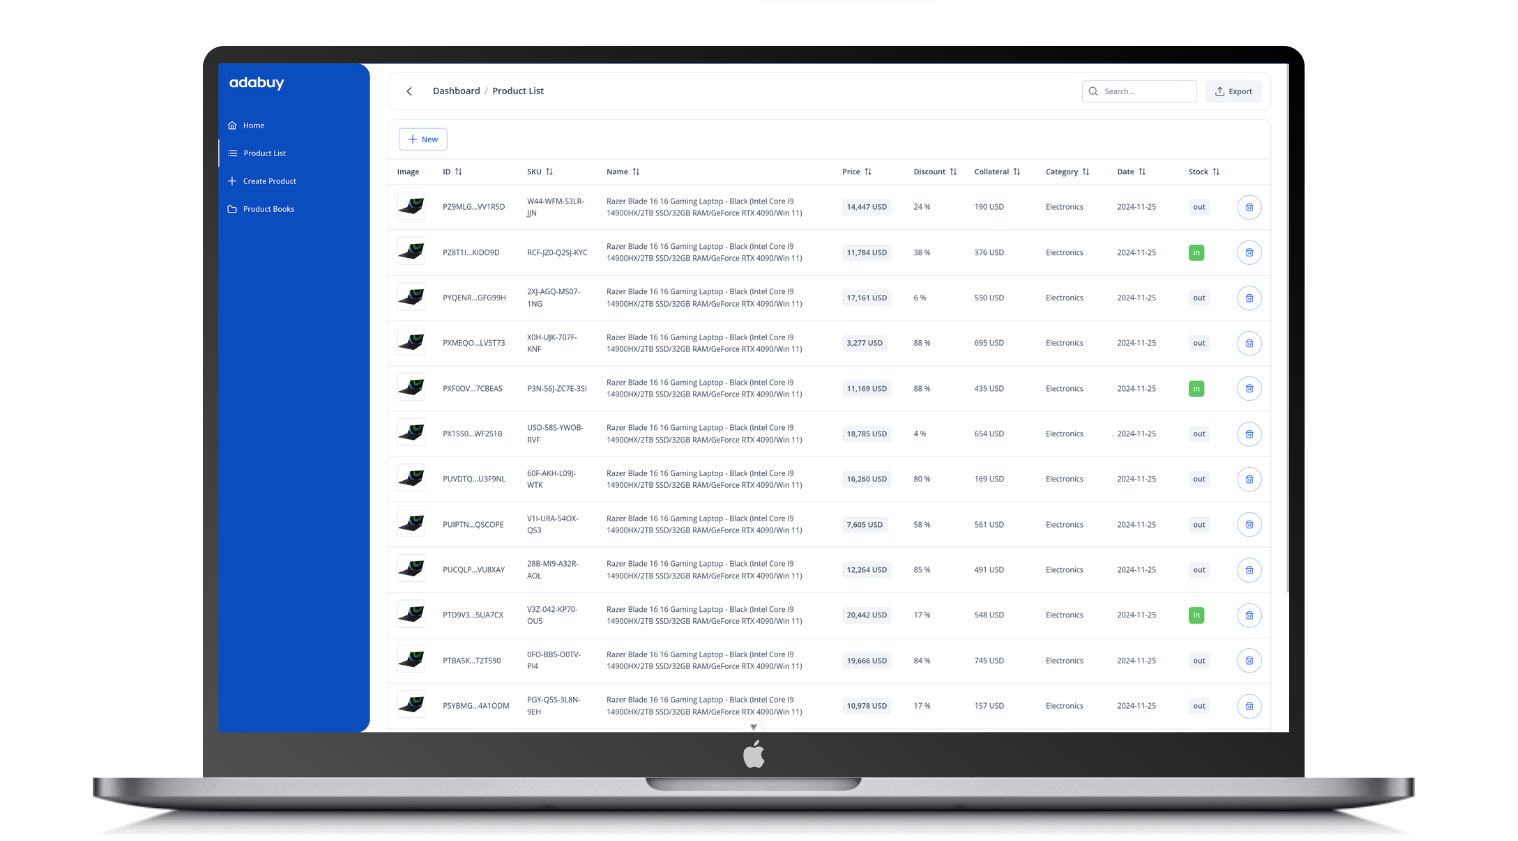
\includegraphics[width=0.88\textwidth, keepaspectratio]{product-list.png}
  \caption{List}
  \label{fig:web}
\end{figure}

\subsubsection { Session } 

When a buyer presses the buy button on a product publication the website redirects them to a single page. The view of a negotiation session contains all the information corresponding to the product, about the seller, the terms of sale, the appeal button, buttons to upload attached images as evidence, alert indications and for the user experience. It also contains live chat to establish bilateral communication between the parties and the mediators.

\subsubsection { Mediators } 

Mediators assigned to a disputed negotiation session will have a special section in the live chat to communicate with the buyer and the seller at the same time. The mediators have no knowledge about the seller and the buyer because they are shown as anonymous digital entities. Mediators cannot be identified by their wallet addresses because they are dynamic addresses changed by the backend.

\subsubsection { Books } 

Product books allow inventory control of products in still stock, ready-to-sell stock, and stock blocked by active purchases. Each book is identified by the stock-keeping-unit (SKU) identifier.

\begin{figure}[ht]
  \centering
  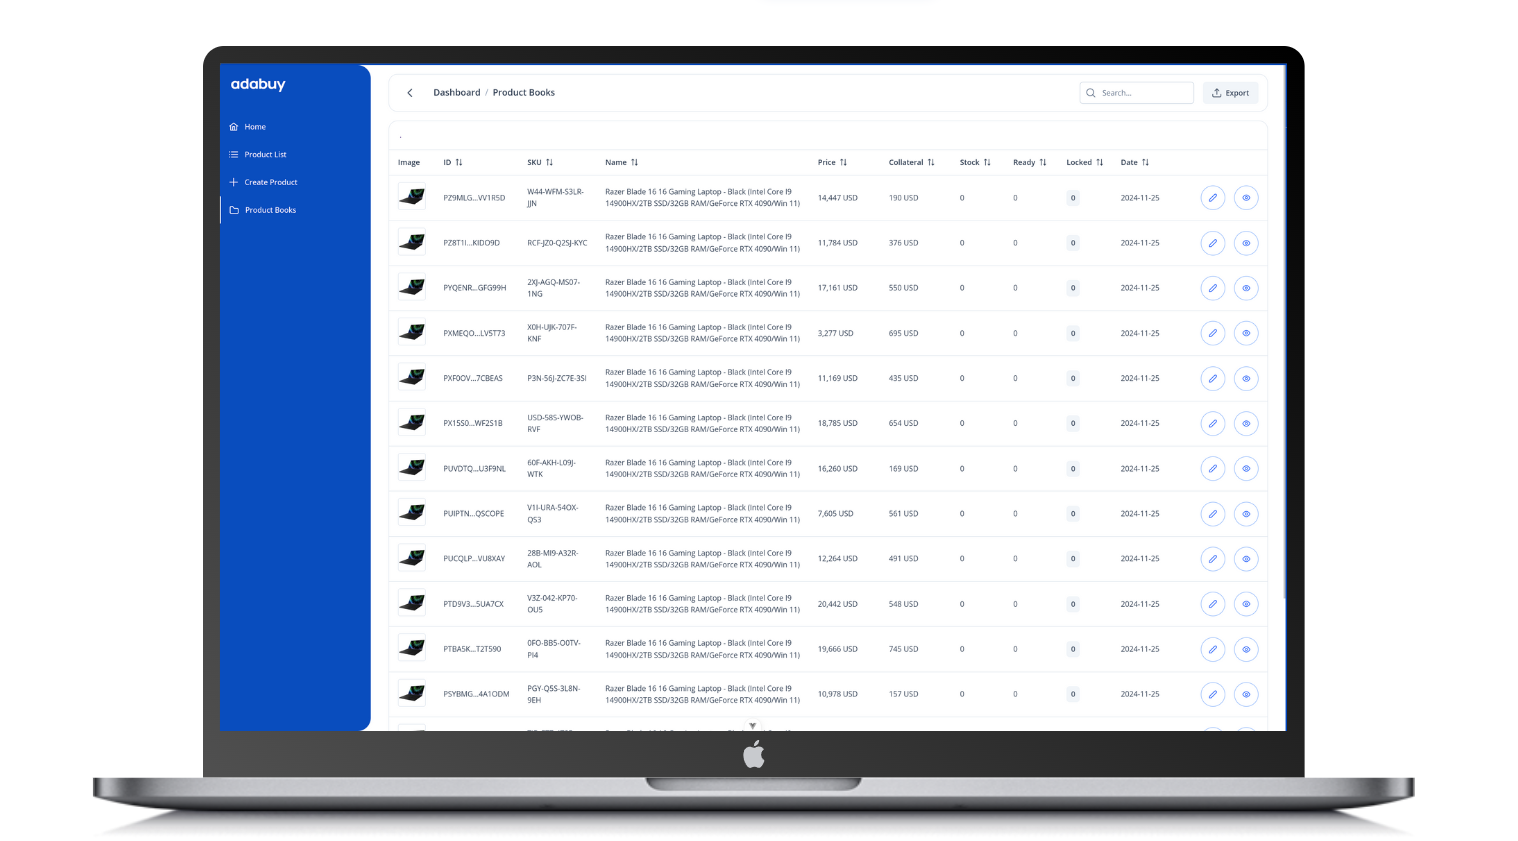
\includegraphics[width=0.88\textwidth, keepaspectratio]{product-books.png}
  \caption{Books}
  \label{fig:web}
\end{figure}

\end{document}
